\documentclass[
11pt, % The default document font size, options: 10pt, 11pt, 12pt
%codirector, % Uncomment to add a codirector to the title page
]{charter} 




% El títulos de la memoria, se usa en la carátula y se puede usar el cualquier lugar del documento con el comando \ttitle
\titulo{Modelo de migración tecnológica para radares} 

% Nombre del posgrado, se usa en la carátula y se puede usar el cualquier lugar del documento con el comando \degreename
%\posgrado{Carrera de Especialización en Sistemas Embebidos} 
%\posgrado{Carrera de Especialización en Internet de las Cosas} 
%\posgrado{Carrera de Especialización en Intelegencia Artificial}
\posgrado{Maestría en Sistemas Embebidos} 
%\posgrado{Maestría en Internet de las cosas}

% Tu nombre, se puede usar el cualquier lugar del documento con el comando \authorname
\autor{Gonzalo Nahuel Vaca} 

% El nombre del director y co-director, se puede usar el cualquier lugar del documento con el comando \supname y \cosupname y \pertesupname y \pertecosupname
\director{Iván Andrés León Vásquez}
\pertenenciaDirector{INVAP S.E.} 
% FIXME:NO IMPLEMENTADO EL CODIRECTOR ni su pertenencia
\codirector{John Doe} % para que aparezca en la portada se debe descomentar la opción codirector en el documentclass
\pertenenciaCoDirector{FIUBA}

% Nombre del cliente, quien va a aprobar los resultados del proyecto, se puede usar con el comando \clientename y \empclientename
\cliente{Andrés Eduardo Monteverde}
\empresaCliente{INVAP S.E.}

% Nombre y pertenencia de los jurados, se pueden usar el cualquier lugar del documento con el comando \jurunoname, \jurdosname y \jurtresname y \perteunoname, \pertedosname y \pertetresname.
\juradoUno{Nombre y Apellido (1)}
\pertenenciaJurUno{pertenencia (1)} 
\juradoDos{Nombre y Apellido (2)}
\pertenenciaJurDos{pertenencia (2)}
\juradoTres{Nombre y Apellido (3)}
\pertenenciaJurTres{pertenencia (3)}
 
\fechaINICIO{29 de junio de 2022}		%Fecha de inicio de la cursada de GdP \fechaInicioName
\fechaFINALPlan{17 de agosto de 2022} 	%Fecha de final de cursada de GdP
\fechaFINALTrabajo{15 de mayo de 2023}	%Fecha de defensa pública del trabajo final


\begin{document}

\maketitle
\thispagestyle{empty}
\pagebreak


\thispagestyle{empty}
{\setlength{\parskip}{0pt}
\tableofcontents{}
}
\pagebreak


\section*{Registros de cambios}
\label{sec:registro}


\begin{table}[ht]
\label{tab:registro}
\centering
\begin{tabularx}{\linewidth}{@{}|c|X|c|@{}}
\hline
\rowcolor[HTML]{C0C0C0} 
Revisión & \multicolumn{1}{c|}{\cellcolor[HTML]{C0C0C0}Detalles de los cambios realizados} & Fecha      \\ \hline
0      & Creación del documento                                 &\fechaInicioName \\ \hline
1      & Se completa el documento salvo el diagrama de GANTT    & 10/07/2022 \\ \hline
%2      & Se completa hasta el punto 7 inclusive
%		  Se puede agregar algo más \newline
%		  En distintas líneas \newline
%		  Así                                                    & dd/mm/aaaa \\ \hline
%3      & Se completa hasta el punto 11 inclusive                & dd/mm/aaaa \\ \hline
%4      & Se completa el plan	                                 & dd/mm/aaaa \\ \hline
\end{tabularx}
\end{table}

\pagebreak



\section*{Acta de constitución del proyecto}
\label{sec:acta}

\begin{flushright}
Buenos Aires, \fechaInicioName
\end{flushright}

\vspace{2cm}

Por medio de la presente se acuerda con el Mg. Ing. \authorname\hspace{1px} que
su Trabajo Final de la \degreename\hspace{1px} se titulará ``\ttitle'',
consistirá esencialmente en la implementación de un prototipo de
  un procesador de datos de radar hecho en Python, y tendrá un presupuesto preliminar estimado de 600 hs de trabajo y \$200, con fecha de inicio \fechaInicioName\hspace{1px} y fecha de presentación pública \fechaFinalName.

Se adjunta a esta acta la planificación inicial.

\vfill

% Esta parte se construye sola con la información que hayan cargado en el preámbulo del documento y no debe modificarla
\begin{table}[ht]
\centering
\begin{tabular}{ccc}
\begin{tabular}[c]{@{}c@{}}Ariel Lutenberg \\ Director posgrado FIUBA\end{tabular} & \hspace{2cm} & \begin{tabular}[c]{@{}c@{}}\clientename \\ \empclientename \end{tabular} \vspace{2.5cm} \\ 
\multicolumn{3}{c}{\begin{tabular}[c]{@{}c@{}} \supname \\ Director del Trabajo Final\end{tabular}} \vspace{2.5cm} \\
%\begin{tabular}[c]{@{}c@{}}\jurunoname \\ Jurado del Trabajo Final\end{tabular}     &  & \begin{tabular}[c]{@{}c@{}}\jurdosname\\ Jurado del Trabajo Final\end{tabular}  \vspace{2.5cm}  \\
%\multicolumn{3}{c}{\begin{tabular}[c]{@{}c@{}} \jurtresname\\ Jurado del Trabajo Final\end{tabular}} \vspace{.5cm}                                                                     
\end{tabular}
\end{table}




\section{1. Descripción técnica-conceptual del proyecto a realizar}
\label{sec:descripcion}

El proyecto a realizar tiene como cliente al Departamento de ingeniería de
software (DISW) de INVAP S.E. en el marco de la Gerencia de gobierno y defensa.

En la cartera de productos de la empresa se pueden encontrar radares
meteorológicos, de vigilancia primarios y secundarios.
Estos equipos generan un gran volumen de datos que deben ser procesados por
algoritmos complejos con la finalidad de obtener información útil.

Los algoritmos son generados por profesionales especializados en la naturaleza
física y matemática del problema y entregan como producto un modelo de
procesamiento de datos en Python.
Luego, el modelo debe correr dentro de un sistema embebido multiprocesador
asimétrico (MPSoC).
Entonces, se procede a traducir el código al lenguaje de programación C para
lograr su compilación en la arquitectura objetivo.

La traducción del modelo genera los siguientes inconvenientes:

\begin{itemize}
  \item Duplicación de tareas.
  \item Dificultad para depurar: se torna difícil determinar si un
    comportamiento erróneo es producto del diseño del modelo o su traducción al
    lenguaje C.
  \item Baja de confiabilidad: la traducción del código es una fuente de
    posibles errores en el sistema.
\end{itemize}

Con la intención de atenuar estos problemas, se deberá realizar un prototipo que
utilice el algoritmo hecho en Python sin traducir. Esto tendría el beneficio
adicional de aliviar la demanda de programadores C/C++ y buscar personal en una
población mayor.

El proyecto se realizará en un \emph{System on chip} (SoC) Zynq-7000 del fabricante
AMD/Xilinx y tendrá los siguientes componentes:

\begin{itemize}
  \item Generador de datos de radar: se deberá sintetizar en la lógica
    programable del integrado.
  \item Modelo procesador: tendrá que estar realizado en Python y podrá ser
    configurado desde el exterior.
  \item Generador de mensajes ASTERIX: deberá crear los mensajes ASTERIX a
    partir de la información generada.
  \item Generador de telemetría: deberá reportar el estado de funcionamiento
    del sistema con mensajes MQTT.
  \item Backend radar corriendo como servicio.
  \item Creación de una distribución de Linux embebido.
\end{itemize}

En la figura \ref{fig:diagBloques} se puede observar un diagrama en bloques
simplificado del sistema propuesto.

\begin{figure}[htpb]
  \centering 
  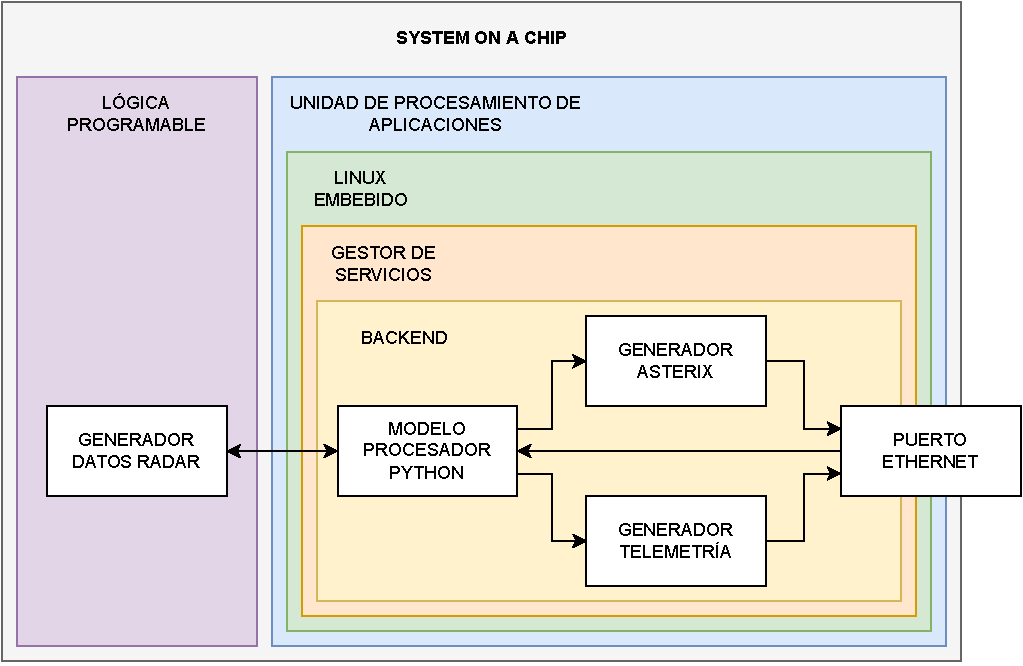
\includegraphics[width=\textwidth]{./Figuras/bloques.pdf}
  \caption{Diagrama en bloques del sistema}
  \label{fig:diagBloques}
\end{figure}


\section{2. Identificación y análisis de los interesados}
\label{sec:interesados}

\begin{table}[ht]
%\caption{Identificación de los interesados}
%\label{tab:interesados}
\begin{tabularx}{\linewidth}{@{}|l|X|X|l|@{}}
\hline
\rowcolor[HTML]{C0C0C0} 
Rol           & Nombre y Apellido & Organización 	  & Puesto \\ \hline
Auspíciate   & Celeste Musso     & \empclientename & Jefa del DISW \\ \hline
Cliente       & \clientename      & \empclientename & Ingeniero de software \\ \hline
Impulsor      & Maximiliano Graf  & \empclientename & Líder de equipo \\ \hline
Responsable   & \authorname       & FIUBA        	  & Alumno \\ \hline
Orientador    & \supname	        & \pertesupname 	& Director del Trabajo final \\ \hline
\end{tabularx}
\end{table}

\section{3. Propósito del proyecto}
\label{sec:proposito}

El propósito de este proyecto es evaluar la posibilidad de realizar un backend
para radares hecho en Python. Con la finalidad de evitar la repetición de
tareas, mejorar la confiabilidad de los sistemas y acceder a una población mayor
de programadores.

\newpage

\section{4. Alcance del proyecto}
\label{sec:alcance}

El presente proyecto incluye:

\begin{itemize}
  \item Crear un esclavo AXI generador de datos de radar.
  \item Crear una distribución de Linux embebido.
  \item Crear un servicio backend radar hecho en Python.
  \item Documentación y manual de usuario.
\end{itemize}

\section{5. Supuestos del proyecto}
\label{sec:supuestos}

Para el desarrollo del presente proyecto se supone que:

\begin{itemize}
	\item Se tendrá acceso a los modelos procesadores de datos de radar.
	\item Se tendrá acceso a una captura de datos de radar.
\end{itemize}

\section{6. Requerimientos}
\label{sec:requerimientos}

A continuación se enumeran los requerimientos del proyecto:

\begin{enumerate}
	\item Requerimientos funcionales
		\begin{enumerate}
      \item El sistema se debe implementar en un SoC de Xilinx.
      \item El sistema debe generar un flujo de datos de radar.
      \item El generador de datos debe ser un esclavo AXI en la lógica programable.
			\item La generación de datos debe ser configurable.
			\item El sistema debe procesar los datos y generar mensajes ASTERIX.
      \item El procesador de datos se debe implementar en Python dentro de la
        Unidad de procesamiento de aplicaciones.
      \item El procesador debe correr como servicio dentro del sistema
        operativo.
      \item Se debe crear una distribución de Linux embebido.
			\item Los mensajes ASTERIX se deben transmitir por protocolo ZMQ.
			\item El sistema debe generar datos de telemetría que indiquen su estado
        de funcionamiento.
			\item La telemetría se debe trasmitir por protocolo MQTT.
			\item El sistema debe presentar una interfaz web para ajustar la
        configuración.
      \item Se debe poder visualizar los mensajes ASTERIX y de telemetría.
		\end{enumerate}
	\item Requerimientos de documentación
		\begin{enumerate}
			\item Se debe generar un informe de rendimiento del procesador de datos implementado.
			\item Se debe crear un manual de uso para el esclavo AXI.
      \item Se debe crear un manual de uso para el servicio procesador de datos.
		\end{enumerate}
	\item Se debe proveer una interfaz web para supervisar y configurar el sistema.
\end{enumerate}

\section{7. Historias de usuarios (\textit{Product backlog})}
\label{sec:backlog}

Las historias de usuario reciben una calificación numérica que refleja la
complejidad de su implementación.
A continuación se detallan los valores posibles:

\begin{itemize}
\item 1 punto: la historia demanda un esfuerzo trivial para satisfacerla.
\item 2 puntos: la historia requiere de conocimientos profundos en una
  tecnología particular.
\item 4 puntos: la historia necesita de conocimientos profundos en más de una tecnología.
\item 8 puntos: la historia demanda múltiples tecnologías y debe cumplir con
  requerimientos de rendimiento.
\item 16 puntos: la historia demanda múltiples tecnologías y debe funcionar en
  tiempo real.
\end{itemize}

A continuación se enumeran las historias de usuario:

\begin{itemize}
  \item Historia 1
    \begin{itemize}
      \item Descripción: como arquitecto de proyectos quiero una interfaz gráfica que me permita
        evaluar el rendimiento del modelo en el sistema embebido.
      \item 8 \emph{History points}: la historia de usuario necesita de
        conocimientos de Python, protocolos ZMQ y HTTP y además se necesita crear
        una página web dentro del sistema embebido. Finalmente, se debe medir el
        rendimiento del sistema.
    \end{itemize}
  \item Historia 2
    \begin{itemize}
      \item Descripción: como desarrollador de la \emph{Radar Computer} necesito obtener
        telemetría MQTT para actualizar el estado del radar.
      \item 4 \emph{History points}: la historia requiere conocimientos de
        programación concurrente en Python y el manejo del protocolo MQTT.
    \end{itemize}
  \item Historia 3
    \begin{itemize}
      \item Descripción: como desarrollador de consolas de radar quiero obtener mensajes en
        formato ASTERIX para poder representar las novedades en campo.
      \item 4 \emph{History points}: se necesitan conocimientos de ZMQ, ASTERIX
        y Python.
    \end{itemize}
\end{itemize}

\section{8. Entregables principales del proyecto}
\label{sec:entregables}

Los entregables del proyecto son:

\begin{itemize}
	\item Manual de usuario del generador de datos.
	\item Manual de usuario del servicio de procesamiento de datos.
	\item Código fuente del generador de datos.
	\item Código fuente del servicio de procesamiento de datos.
	\item Informe de rendimiento del servicio de procesamiento de datos.
\end{itemize}


\section{9. Desglose del trabajo en tareas}
\label{sec:wbs}

\begin{enumerate}
\item Planificación y recursos
	\begin{enumerate}
	\item Creación del documento de planificación (20 hs)
	\item Instalación del ambiente de desarrollo (15 hs)
	\item Creación del repositorio (5 hs)
	\item Gestión de horas (5 hs)
	\item Obtención de un \emph{set} de datos (15 hs)
	\item Obtención de un modelo de procesamiento (15 hs)
	\end{enumerate}
\item Investigación
	\begin{enumerate}
	\item Análisis de dependencias del modelo de procesamiento (15 hs)
	\item Análisis del funcionamiento del modelo de procesamiento (60 hs)
	\item Análisis del \emph{set} de datos (50 hs)
	\end{enumerate}
\item Generador de datos
	\begin{enumerate}
	\item Modelo RTL del encoder absoluto (15 hs)
	\item Simulación, síntesis y depuración del encoder absoluto (15 hs)
	\item Modelo RTL del generador de datos (39 hs)
	\item Simulación, síntesis y depuración del generador de datos (15 hs)
	\item Creación del IP Core (15 hs)
	\item Pruebas del IP Core (25 hs)
	\end{enumerate}
\item Backend radar
	\begin{enumerate}
	\item Creación y prueba del proyecto Petalinux (5 hs)
	\item Compilación y prueba del intérprete de Python (5 hs)
	\item Compilación y prueba de la biblioteca ZMQ (10 hs)
	\item Compilación y prueba de la biblioteca MQTT (5 hs)
	\item Compilación y prueba de la biblioteca FLASK (10 hs)
	\item Desarrollo, compilación y prueba del árbol de dispositivos (15 hs)
	\item Desarrollo, compilación y prueba del driver del generador de datos (40 hs)
	\item Desarrollo, compilación y prueba de la biblioteca ASTERIX (35 hs)
	\item Integración del Backend radar (40 hs)
	\item Pruebas de funcionamiento (20 hs)
	\end{enumerate}
\item Cierre
	\begin{enumerate}
	\item Creación del manual del generador de datos (5 hs)
	\item Creación del manual del Backend radar (5 hs)
	\item Creación del informe de rendimiento del sistema (30 hs)
	\item Creación de la memoria del Trabajo Final (10 hs)
	\item Creación de un vídeo de demostración (10 hs)
	\item Defensa pública y agradecimientos (1 hs)
	\end{enumerate}
\end{enumerate}

Cantidad total de horas: 600 hs.


\section{10. Diagrama de Activity On Node}
\label{sec:AoN}

\begin{figure}[H]
\centering 
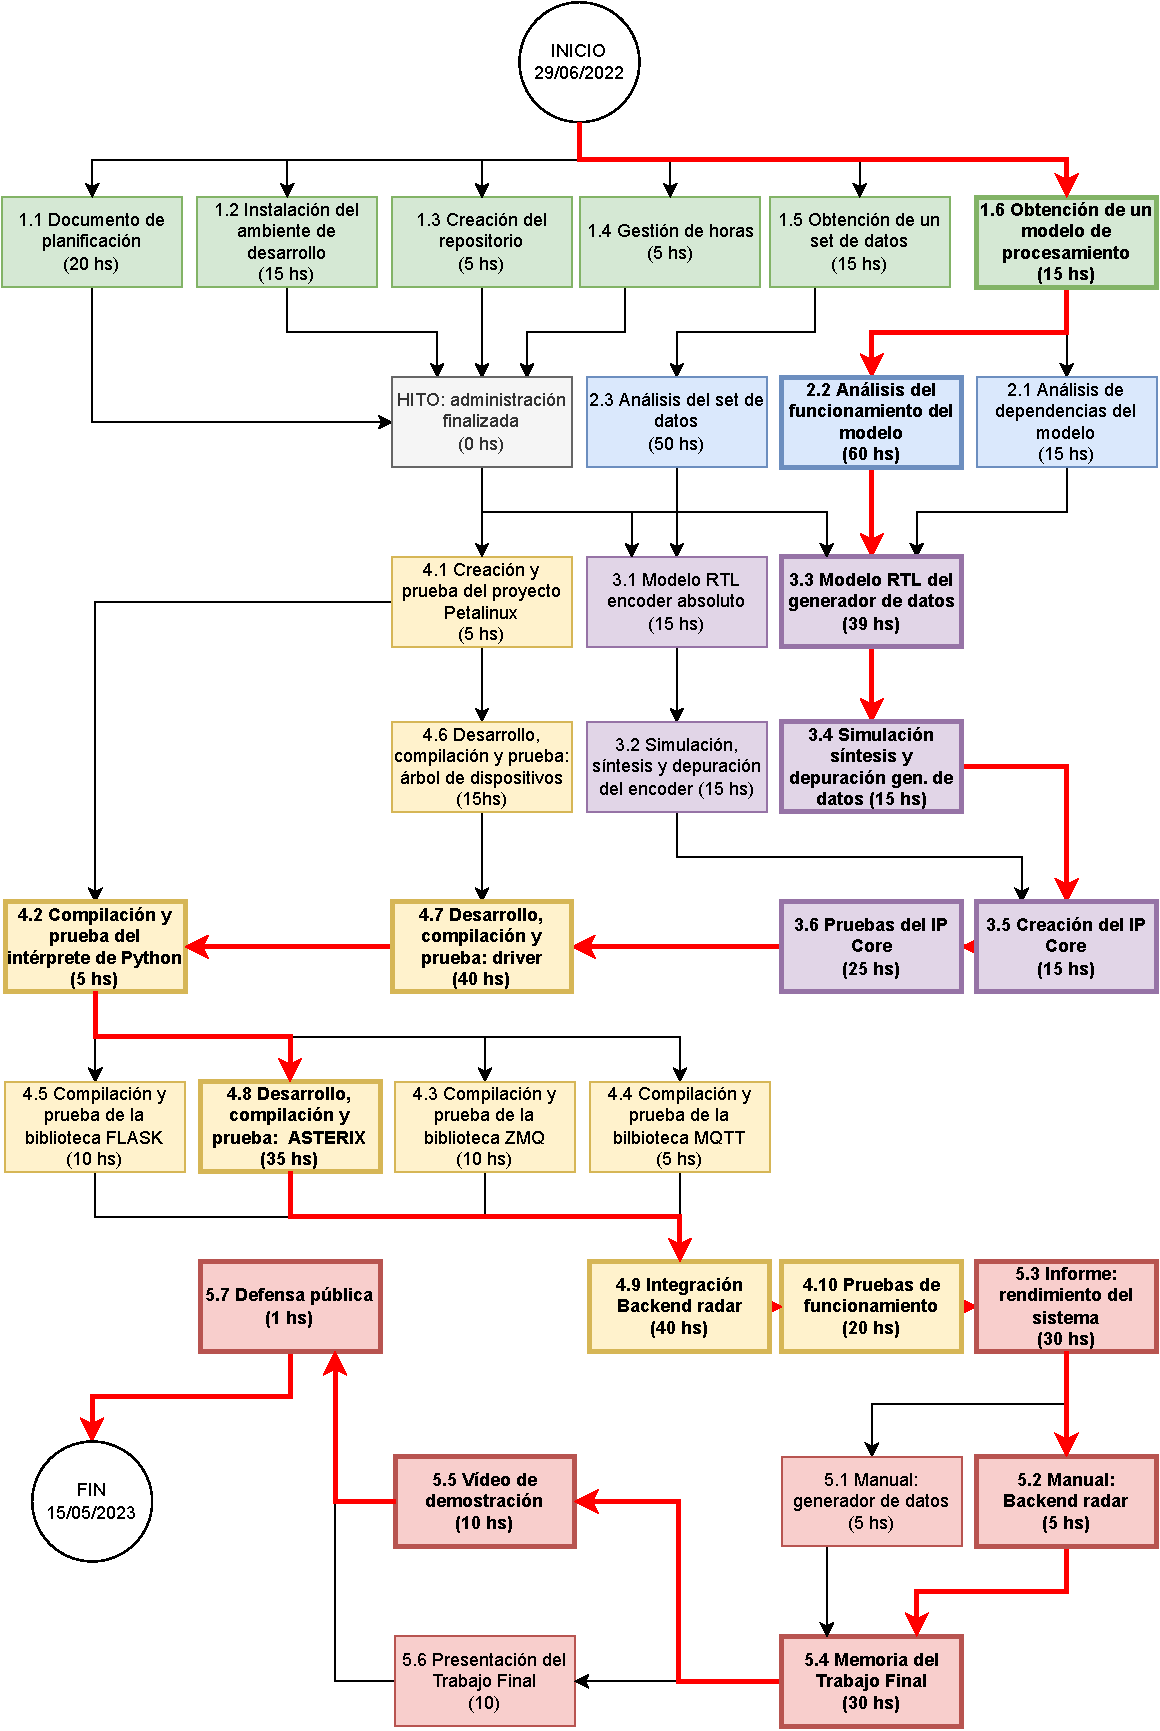
\includegraphics[width=.9\textwidth]{./Figuras/AoN.pdf}
\caption{Diagrama en \textit{Activity on Node}}
\label{fig:AoN}
\end{figure}

\section{11. Diagrama de Gantt}
\label{sec:gantt}

\begin{consigna}{red}

Existen muchos programas y recursos \textit{online} para hacer diagramas de gantt, entre los cuales destacamos:

\begin{itemize}
\item Planner
\item GanttProject
\item Trello + \textit{plugins}. En el siguiente link hay un tutorial oficial: \\ \url{https://blog.trello.com/es/diagrama-de-gantt-de-un-proyecto}
\item Creately, herramienta online colaborativa. \\\url{https://creately.com/diagram/example/ieb3p3ml/LaTeX}
\item Se puede hacer en latex con el paquete \textit{pgfgantt}\\ \url{http://ctan.dcc.uchile.cl/graphics/pgf/contrib/pgfgantt/pgfgantt.pdf}
\end{itemize}

Pegar acá una captura de pantalla del diagrama de Gantt, cuidando que la letra sea suficientemente grande como para ser legible. 
Si el diagrama queda demasiado ancho, se puede pegar primero la ``tabla'' del Gantt y luego pegar la parte del diagrama de barras del diagrama de Gantt.

Configurar el software para que en la parte de la tabla muestre los códigos del EDT (WBS).\\
Configurar el software para que al lado de cada barra muestre el nombre de cada tarea.\\
Revisar que la fecha de finalización coincida con lo indicado en el Acta Constitutiva.

En la figura \ref{fig:gantt}, se muestra un ejemplo de diagrama de gantt realizado con el paquete de \textit{pgfgantt}. En la plantilla pueden ver el código que lo genera y usarlo de base para construir el propio.

\begin{figure}[htbp]
\begin{center}
\begin{ganttchart}{1}{12}
  \gantttitle{2020}{12} \\
  \gantttitlelist{1,...,12}{1} \\
  \ganttgroup{Group 1}{1}{7} \\
  \ganttbar{Task 1}{1}{2} \\
  \ganttlinkedbar{Task 2}{3}{7} \ganttnewline
  \ganttmilestone{Milestone o hito}{7} \ganttnewline
  \ganttbar{Final Task}{8}{12}
  \ganttlink{elem2}{elem3}
  \ganttlink{elem3}{elem4}
\end{ganttchart}
\end{center}
\caption{Diagrama de gantt de ejemplo}
\label{fig:gantt}
\end{figure}


\begin{landscape}
\begin{figure}[htpb]
\centering 
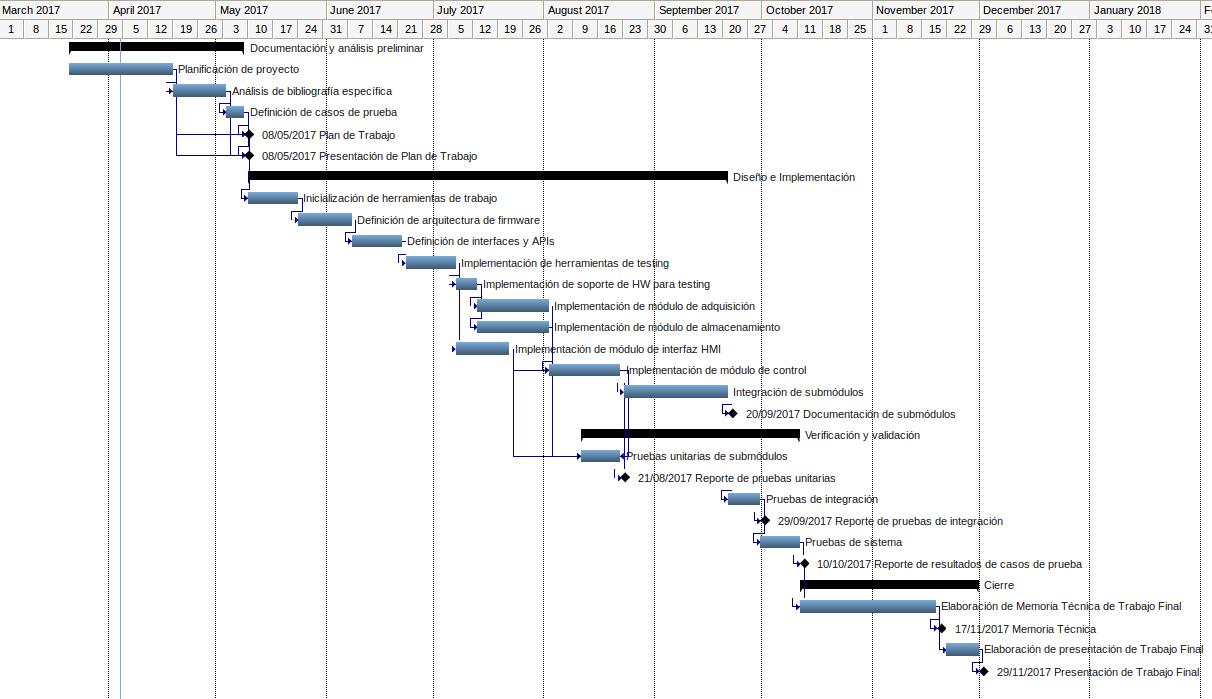
\includegraphics[height=.85\textheight]{./Figuras/Gantt-2.png}
\caption{Ejemplo de diagrama de Gantt rotado}
\label{fig:diagGantt}
\end{figure}

\end{landscape}

\end{consigna}


\section{12. Presupuesto detallado del proyecto}
\label{sec:presupuesto}

A continuación se detallan los costos previstos para del proyecto:

\begin{table}[htpb]
\centering
\begin{tabularx}{\linewidth}{@{}|X|c|r|r|@{}}
\hline
\rowcolor[HTML]{C0C0C0} 
\multicolumn{4}{|c|}{\cellcolor[HTML]{C0C0C0}COSTOS DIRECTOS} \\ \hline
\rowcolor[HTML]{C0C0C0} 
Descripción &
  \multicolumn{1}{c|}{\cellcolor[HTML]{C0C0C0}Cantidad} &
  \multicolumn{1}{c|}{\cellcolor[HTML]{C0C0C0}Valor unitario} &
  \multicolumn{1}{c|}{\cellcolor[HTML]{C0C0C0}Valor total} \\ \hline
  Arty Z7&
  \multicolumn{1}{c|}{1} &
  \multicolumn{1}{c|}{USD 200} &
  \multicolumn{1}{c|}{USD 200} \\ \hline
%   &
%  \multicolumn{1}{c|}{} &
%  \multicolumn{1}{c|}{} &
%  \multicolumn{1}{c|}{} \\ \hline
%\multicolumn{1}{|l|}{} &
%   &
%   &
%   \\ \hline
%\multicolumn{1}{|l|}{} &
%   &
%   &
%   \\ \hline
\multicolumn{3}{|c|}{SUBTOTAL} &
  \multicolumn{1}{c|}{USD 200} \\ \hline
\rowcolor[HTML]{C0C0C0} 
\multicolumn{4}{|c|}{\cellcolor[HTML]{C0C0C0}COSTOS INDIRECTOS} \\ \hline
\rowcolor[HTML]{C0C0C0} 
Descripción &
  \multicolumn{1}{c|}{\cellcolor[HTML]{C0C0C0}Cantidad} &
  \multicolumn{1}{c|}{\cellcolor[HTML]{C0C0C0}Valor unitario} &
  \multicolumn{1}{c|}{\cellcolor[HTML]{C0C0C0}Valor total} \\ \hline
  \multicolumn{1}{|l|}{Costos de aduana} &
  1 &
  USD 100 &
  USD 100
   \\ \hline
%\multicolumn{1}{|l|}{} &
%   &
%   &
%   \\ \hline
%\multicolumn{1}{|l|}{} &
%   &
%   &
%   \\ \hline
\multicolumn{3}{|c|}{SUBTOTAL} &
  \multicolumn{1}{c|}{USD 100} \\ \hline
\rowcolor[HTML]{C0C0C0}
\multicolumn{3}{|c|}{TOTAL} &
  USD 300 \\ \hline
\end{tabularx}%
\end{table}


\section{13. Gestión de riesgos}
\label{sec:riesgos}

a) A continuación se identifican los riesgos previstos en el proyecto:

Riesgo 1: demoras en la adquisición del hardware.
\begin{itemize}
\item Severidad (4): no es posible realizar pruebas de rendimiento sin tener el
  hardware real, sin embargo es posible realizar el desarrollo del proyecto.
\item Probabilidad de ocurrencia (7): es frecuente tener problemas para realizar
  importaciones en la República Argentina. 
\end{itemize}   

Riesgo 2: sin acceso al algoritmo desarrollado por modelística.
\begin{itemize}
\item Severidad (10): sin el modelo no es posible realizar el proyecto.
\item Ocurrencia (1): el proyecto tiene el apoyo de la jefa del departamento de
  ingeniería de software.
\end{itemize}

Riesgo 3: sin acceso a una colección de datos de radar.
\begin{itemize}
\item Severidad (7): sin datos reales de radar se pierde la posibilidad
  de realizar pruebas que arrojen resultados útiles.
\item Ocurrencia (1): el proyecto tiene el apoyo de la jefa del departamento de
  ingeniería de software.
\end{itemize}

Riesgo 4: sin horas para realizar el proyecto durante el horario laboral.
\begin{itemize}
\item Severidad (5): el proyecto contempla el uso de horas dentro del horario
  laboral para cumplir con la fecha de entrega.
\item Ocurrencia (5): las obligaciones contractuales de la empresa pueden forzar
  la eliminación de las horas otorgadas para el proyecto.
\end{itemize}

Riesgo 5: imposibilidad económica para continuar el posgrado.
\begin{itemize}
\item Severidad (10): Significaría el fin del proyecto.
\item Ocurrencia (1): Se tienen los recursos económicos necesarios para cursar
  los cinco bimestres.
\end{itemize}


b) Tabla de gestión de riesgos:      (El RPN se calcula como RPN=SxO)

\begin{table}[htpb]
\centering
\begin{tabularx}{\linewidth}{@{}|X|c|c|c|c|c|c|@{}}
\hline
\rowcolor[HTML]{C0C0C0} 
Riesgo                                                         & S & O & RPN & S* & O* & RPN* \\ \hline
Demoras en la adquisición del hardware                         & 4 & 7 &  28 & 1  & 7  &  7   \\ \hline
Sin acceso al algoritmo desarrollado por modelística           &10 & 1 &  10 &    &    &      \\ \hline
Sin acceso a una colección de datos de radar                   & 7 & 1 &   7 &    &    &      \\ \hline
Sin horas para realizar el proyecto durante el horario laboral & 5 & 5 &  25 & 2  & 5  &  10  \\ \hline
Imposibilidad económica para continuar el posgrado             &10 & 1 &  10 &    &    &      \\ \hline
\end{tabularx}%
\end{table}

Criterio adoptado: 
Se tomarán medidas de mitigación en los riesgos cuyos números de RPN sean
mayores a 20.

Nota: los valores marcados con (*) en la tabla corresponden luego de haber aplicado la mitigación.

c) Plan de mitigación de los riesgos que originalmente excedían el RPN máximo establecido:
 
Riesgo 1: se pone a disposición del proyecto hardware que es propiedad del
responsable del proyecto. \\
  - Severidad (1): al disponer del hardware del responsable del proyecto se
  elimina los efectos negativos asociados al riesgo.\\
  - Probabilidad de ocurrencia (7): la mitigación adoptada no altera la
  probabilidad de ocurrencia.

Riesgo 4: el responsable del proyecto planifica su agenda personal para tener a
disposición las horas necesarias.\\
  - Severidad (2): al disponer de horas libres en la agenda del responsable del
  proyecto se atenúa el efecto negativo del riesgo.\\
  - Probabilidad de ocurrencia (7): la mitigación adoptada no altera la
  probabilidad de ocurrencia.

\section{14. Gestión de la calidad}
\label{sec:calidad}

\begin{itemize}
	\item Requerimientos funcionales
		\begin{itemize}
      \item REQ-01: el sistema se debe implementar en un SoC de Xilinx.
        \begin{itemize}
          \item Verificación: se correrá el sistema en QEMU para luego ser probado
          en la placa Arty Z7. 
          \item Validación: se le mostrará al cliente la ejecución del sistema en
          la placa Arty Z7.  
        \end{itemize}
      \item REQ-02: el sistema debe generar un flujo de datos de radar.
        \begin{itemize}
          \item Verificación: se realizará un \emph{script} que capture el flujo
            de datos y los compare con los valores esperados.
          \item Validación: se realizará un \emph{script} que envíe los datos
            por protocolo UDP para que el cliente pueda realizar sus propias
            pruebas.
        \end{itemize}
      \item REQ-03: el generador de datos debe ser un esclavo AXI en la lógica
        programable.
        \begin{itemize}
          \item Verificación: se correrán las pruebas automáticas del entorno de
            desarrollo integrado Vivado.
          \item Validación: Se generará un \emph{IP Core} para que el cliente
            realice sus propias pruebas.
        \end{itemize}
			\item REQ-04: la generación de datos debe ser configurable.
        \begin{itemize}
          \item Verificación: se realizará una demostración en donde se cambiará
            la velocidad de barrido en azimut y se designarán zonas inhibidas.
          \item Validación: el cliente entregará una serie de configuraciones
            durante la demostración y se persistirán los resultados para que el
            cliente decida si el generador funciona de forma correcta.
        \end{itemize}
			\item REQ-05: el sistema debe procesar los datos y generar mensajes
        ASTERIX.
        \begin{itemize}
          \item Verificación: se usará un programa del tipo \emph{parser} que
            determina si el protocolo se usó de forma correcta.
          \item Validación: se entregará una captura de mensajes ASTERIX al
            cliente.
        \end{itemize}
      \item REQ-06: el procesador de datos se debe implementar en Python dentro de la
        Unidad de procesamiento de aplicaciones.
        \begin{itemize}
          \item Verificación: se relevará la proporción de lenguajes en la
            aplicación.
          \item Validación: se realizará un control de versiones en un
            repositorio dentro de la infraestructura de INVAP S.E.
        \end{itemize}
      \item REQ-07: el procesador debe correr como servicio dentro del sistema
        operativo.
        \begin{itemize}
          \item Verificación: se realizará un \emph{boot} del \emph{kernel} y se
            mostrará el mensaje del sistema operativo que muestra el inicio del
            servicio.
          \item Validación: con el sistema operativo funcionando se pedirá la
            lista de procesos y debe figurar el servicio.
        \end{itemize}
      \item REQ-08: se debe crear una distribución de Linux embebido.
        \begin{itemize}
          \item Verificación: se realizará una demostración de \emph{boot} de la
            distribución.
          \item Validación: el proyecto Petalinux estará en un repositorio
            dentro de la infraestructura de INVAP S.E.
        \end{itemize}
			\item REQ-09: los mensajes ASTERIX se deben transmitir por protocolo ZMQ.
        \begin{itemize}
          \item Verificación: se usará un cliente ZMQ para recibir los datos.
          \item Validación: se realizará una demostración de la captura de datos
            en ZMQ.
        \end{itemize}
			\item REQ-10: el sistema debe generar datos de telemetría que indiquen su estado
        de funcionamiento.
        \begin{itemize}
          \item Verificación: se inducirán fallas en el sistema y se deberán
            reflejar en la telemetría.
          \item Validación: se repetirá el ensayo de verificación pero el
            cliente será quién decida que componentes se pondrán en falla.
        \end{itemize}
			\item REQ-11: la telemetría se debe trasmitir por protocolo MQTT.
        \begin{itemize}
          \item Verificación: se usará un cliente MQTT para capturar la
            telemetría.
          \item Validación: se repetirá la prueba de verificación en presencia
            del cliente.
        \end{itemize}
			\item REQ-12: el sistema debe presentar una interfaz web para ajustar la
        configuración.
        \begin{itemize}
          \item Verificación: se realizarán cambios desde la interfaz web y se
            verá el impacto en el archivo de configuración.
          \item Validación: se realizarán cambios desde la interfaz web y se
            verá el cambio de comportamiento en el sistema.
        \end{itemize}
      \item REQ-13: se debe poder visualizar los mensajes ASTERIX y de
        telemetría.
        \begin{itemize}
          \item Verificación: se generarán mensajes de pruebas en ASTERIX y MQTT
            y se medirá su impacto en la interfaz gráfica.
          \item Validación: se pondrá el sistema en funcionamiento y se medirá
            su impacto en la interfaz gráfica.
        \end{itemize}
		\end{itemize}
	\item Requerimientos de documentación
		\begin{itemize}
      \item REQ-14: se debe generar un informe de rendimiento del procesador de
        datos implementado.
        \begin{itemize}
          \item Verificación: se cambiará la velocidad de giro del generador de
            datos y se estudiará cuantos paquetes se pierden en cada caso.
          \item Validación: se conectará el sistema a una consola de radar y se
            probarán distintas configuraciones del generador de datos.
        \end{itemize}
      \item REQ-15: se debe crear un manual de uso para el esclavo AXI.
        \begin{itemize}
          \item Verificación: se creará un proyecto nuevo y se seguirán los
            pasos especificados en el manual, el resultado debe ser una
            aplicación de ejemplo que funcione.
          \item Validación: el cliente realizará una revisión del documento.
        \end{itemize}
      \item REQ-16: se debe crear un manual de uso para el servicio procesador de datos.
        \begin{itemize}
          \item Verificación: se creará un proyecto nuevo y se seguirán los
          pasos especificados en el manual, el resultado debe ser una
          aplicación de ejemplo que funcione.
          \item Validación: el cliente realizará una revisión del documento.
        \end{itemize}
      \end{itemize}
    \item REQ-17: se debe proveer una interfaz web para supervisar y configurar el sistema.
      \begin{itemize}
        \item Verificación: se realizará un \emph{log} de los pedidos
          provenientes de la interfaz web para analizar su correcto funcionamiento.
        \item Validación: el cliente probará la interfaz web y dará sus correcciones.
      \end{itemize}
\end{itemize}

\section{15. Procesos de cierre}    
\label{sec:cierre}

Establecer las pautas de trabajo para realizar una reunión final de evaluación del proyecto, tal que contemple las siguientes actividades:

\begin{itemize}
	\item Pautas de trabajo que se seguirán para analizar si se respetó el Plan de Proyecto original:
        \begin{itemize}
            \item El responsable del proyecto analizará el plan original y se verificará el grado de correspondencia con su ejecución.
            \item El responsable del proyecto evaluará las tareas que no se ajustaron al plan para detectar las causas y tenerlas en cuentas en próximos proyectos.
	    \end{itemize}

    \item Identificación de las técnicas y procedimientos útiles e inútiles que se emplearon, y los problemas que surgieron y cómo se solucionaron:
	    \begin{itemize}
            \item El responsable del proyecto evaluará el rendimiento del
              lenguaje de programación Python en un backend radar.
            \item El responsable del proyecto generará informes con todos los problemas técnicos no previstos.
        \end{itemize}
	\item Luego de la presentación del trabajo ante el jurado, el responsable del proyecto realizará un agradecimiento público a todas las personas involucradas en el proyecto. 
\end{itemize}

\end{document}
